\section{Human-Inspired Control}
\showtoc

\subsection{Human-Inspired Control Framework}
\frame{
  \frametitle{Human Data Experiment}
  \begin{columns}
    \begin{column}{0.65\textwidth}
      \begin{figure}
        \centering
        \vspace{-1cm}
        \caption{Experimental setup showing sensor placement for human data acquisition}
        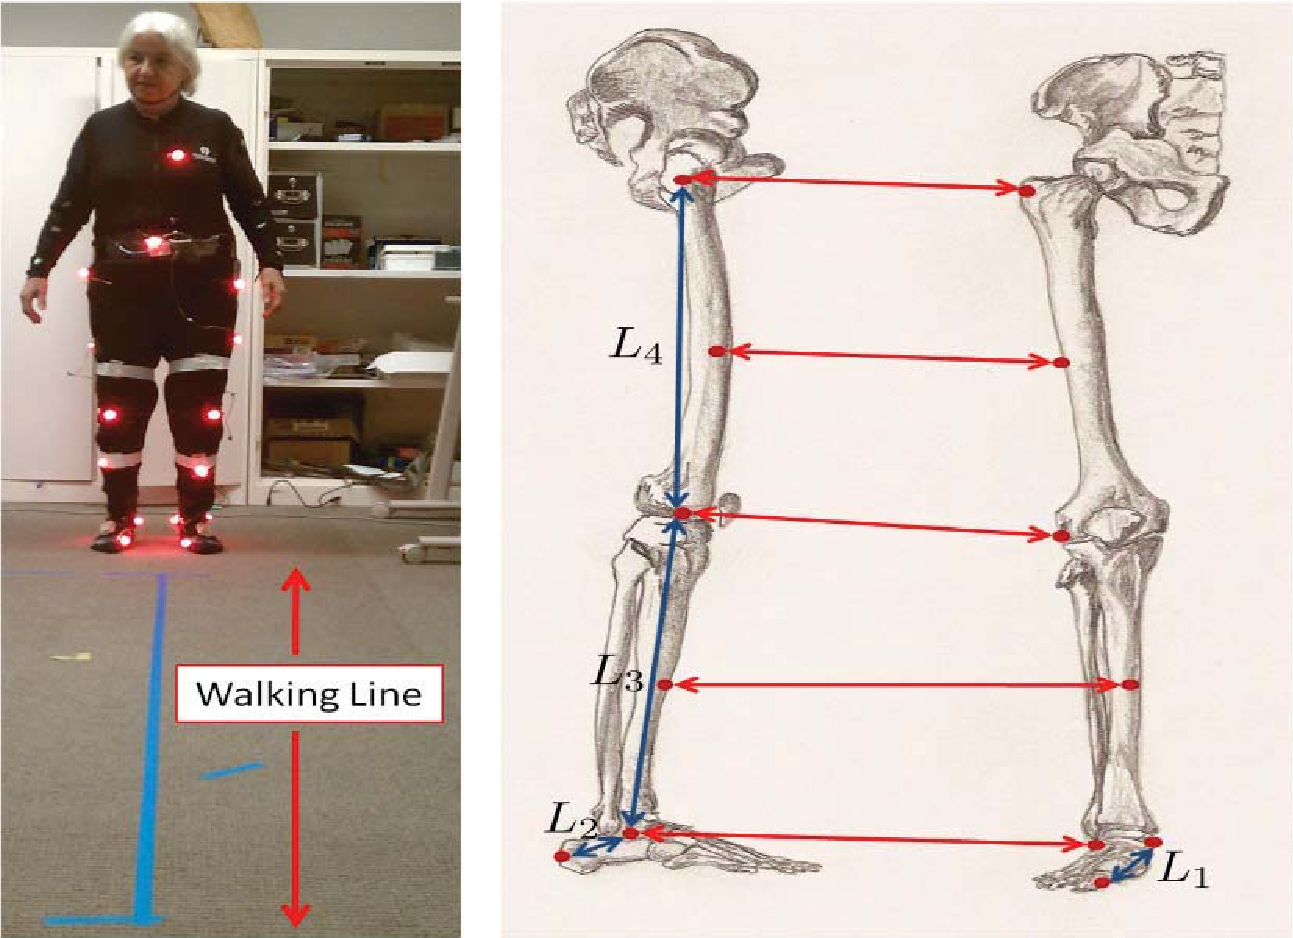
\includegraphics[width=1.0\columnwidth]{labeled_diagram}
      \end{figure}
    \end{column}
    \begin{column}{0.35\textwidth}
      \begin{figure} \centering
        \vspace{-1cm}
        \caption{Human outputs}
        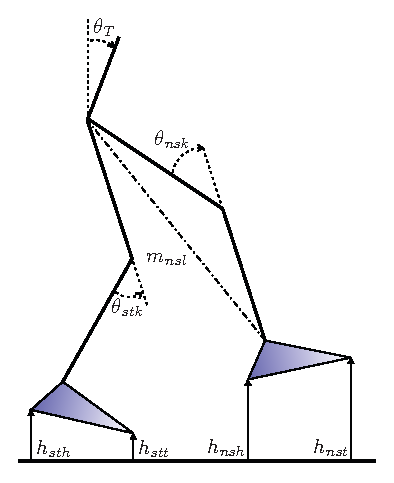
\includegraphics[width=0.8\columnwidth]{robot_const}
      \end{figure}
    \end{column}
  \end{columns}
}

\frame[t]{
  \frametitle{Canonical Walking Functions}
  The following function, termed the \blue{canonical walking function}, fits human kinematics data quite accurately:
  \begin{align}
    \nonumber
    y(t) &= e^{-\zeta \omega_{n} t} (c_{1} \cos (\omega_{d} t) + c_{2} \sin (\omega_{d} t)) + \hat{g}\\
    \tag{CWF}
    \label{eq:cwf}
    y^{H}(t, A)&= e^{-a_{3} t} (a_{1} \cos (a_{2} t) + a_{4} \sin (a_{2} t)) + a_{5}
  \end{align}
  where,
  \begin{itemize}
  \item
    $\zeta$ is the damping ratio,
  \item
    $\omega_{n}$, $\omega_{d}$ are the natural and damped natural frequencies, resp.,
  \item
    $c_{1}$ and $c_{2}$ are initial conditions,
  \item
    and $\hat{g}$ is from a particular solution for constant forcing.
  \end{itemize}
  Parameterize time using hip position:
  \begin{align*}
    \tau(\theta) := \frac{p_\mathit{hip}^{x}(\theta) - p_\mathit{hip}^{x}(\theta^{-})}{v_\mathit{hip}}
  \end{align*}
}

\begin{frame}
  \frametitle{Example: 5-Link Biped}
  \begin{columns}
    \column{1.5in}
    Dynamic Model:
    \begin{align*}
      M(q) \ddot q + H(q, \dot q) = 0
    \end{align*}
    \column{1.5in}
    \begin{figure}
      \centering
      \def\svgwidth{1.0\columnwidth}
      \input{figures/cg2d-5link-model.eps_latex}
      \vspace{-2em}
      \caption{5-link biped configuration.}
    \end{figure}
  \end{columns}
\end{frame}

\frame{
  \frametitle{Selecting Human Outputs}
  The following human kinematics outputs are viable:
  \begin{enumerate}
    {
    \item[\HF{1}:] $\Oa$, \blue{forward hip velocity}, i.e., the velocity of the $x$-position of the hip,
    \item[\HF{2}:] $\Ob$, \blue{swing leg slope}, i.e., the tangent of the angle between the $z$-axis and the projection of the line connecting the swing ankle and hip,
    \item[\HF{3}:] $\Oc$, \blue{stance knee relative angle},
    \item[\HF{4}:] $\Od$, \blue{swing knee relative angle},
    \item[\HF{5}:] $\Oe$, \blue{vertical torso angle}, the angle of the torso measured with respect to the vertical axis of the world frame.
    }
  \end{enumerate}

  \vspace{1mm}
  For convenience, define the actual and desired outputs:
  \vspace{-1mm}
  \begin{align*}
    y_{1}^{a} = \Oa, \ y_{2}^{a} = \Ob, \ y_{3}^{a} = \Oc, \ y_{4}^{a} = \Od, \ y_{5}^{a} = \Oe,
  \end{align*}
  \vspace{-8mm}
  \begin{align*}
    y_{1}^{d} = y^{H}(\tau(\theta), A_1), \ \ldots, \ y_{5}^{d} = y^{H}(\tau(\theta), A_5)
  \end{align*}
}

\frame{
  \frametitle{Human-Inspired Optimization}
  The form of \eqref{eq:cwf} allows it to encode certain outputs:
  \vspace{-4mm}
  \begin{figure}
    \centering
    \caption{Canonical walking functions with parameters from \eqref{eq:opt}}
    \vspace{-2mm}
    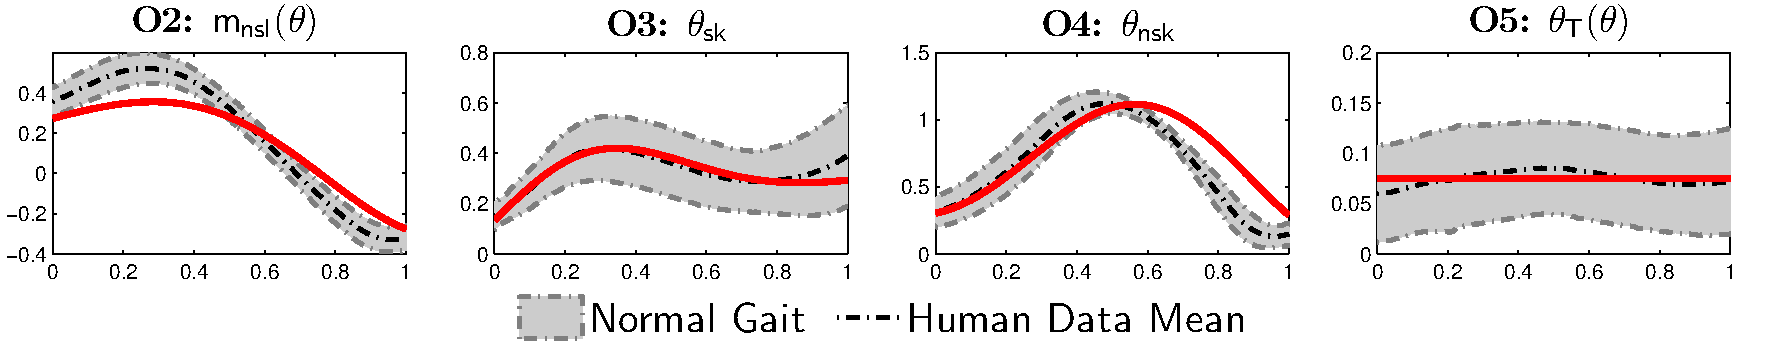
\includegraphics[width=1.0\textwidth]{human_function_fits}
    \vspace{-2mm}
  \end{figure}
  These outputs can be used to construct a \blue{partial hybrid zero dynamics} parameterized by matrix $A$ where outputs \textcolor{blue}{\HF{2}}--\textcolor{blue}{\HF{5}} of the robot are equal to the desired outputs for all time. The optimal parameters $A^*$ are found by solving
  \begin{align}
    \label{eq:opt}
    \tag{$\mathcal{O}$}
    A^{*} = \underset{A \in \R^{5 \times 5}}{\operatorname{argmin}} &  \:\: \mathrm{Cost}_{\mathrm{HD}}(A)  \\[-1mm]
    \nonumber
    \mathrm{s.t.} \quad & \ResetMapReduced(\GuardReduced \cap \HZD_{A}) \subset \PHZD_{A}
  \end{align}
}

\begin{frame}
  \frametitle{Tracking the Partial Hybrid Zero Dynamics}
  Tracking can be accomplished with a variety of control schemes. PD control is interesting due to its model-independent nature:
  \begin{align*}
    \mathcal{K}_{2D}(\theta, \dot{\theta}) \! = \! k_p \left(\!\!
    \begin{array}{c}
      0\\
      y_{d,2} - y_{a,2}\\
      y_{d,3} - y_{a,3}\\
      y_{d,4} - y_{a,4}\\
      y_{d,5} - y_{a,5}
    \end{array}\!\!\right)  + 
    \blkdiag (k_p, k_d I_4)\left(\!\!
    \begin{array}{c}
      y_{d,1} - y_{a,1}\\
      \dot{y}_{d,2} - \dot{y}_{a,2}\\
      \dot{y}_{d,3} - \dot{y}_{a,3}\\
      \dot{y}_{d,4} - \dot{y}_{a,4}\\
      \dot{y}_{d,5} - \dot{y}_{a,5}
    \end{array}\!\!\right)
  \end{align*}

  This control law will result in walking in simulation (and in experiment in other works) and will satisfy assumptions made by functional Routhian reduction (introduced later).
\end{frame}

\begin{frame}
  \frametitle{Procedure Summary}
  \begin{figure}
    \includemedia[
      width=0.8\columnwidth,
      height=0.45\columnwidth,
      addresource=human_experiment.mp4,
      activate=pageopen,
      flashvars={source=human_experiment.mp4&loop=true&autoPlay=true}
    ]{}{VPlayer9.swf}
    \caption{Human-inspired control produces robotic gaits from human data.}
  \end{figure}
\end{frame}

\begin{frame}
  \frametitle{3D Simulation Results}
  \only<1>{
    \begin{figure}
      \centering
      \caption{Walking gait for 3D model with $v_\mathit{hip} = .6$ m/s}
      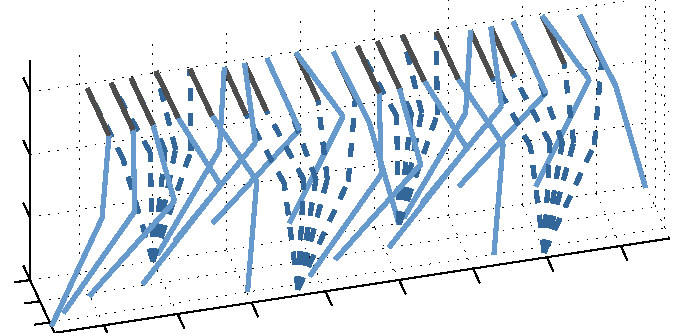
\includegraphics[width=.9\textwidth]{hic_frr_tiles_3d}
    \end{figure}
  }
  \only<2>{
    \begin{figure}
      \centering
      \caption{Phase portraits, human outputs, and actuator torques}
      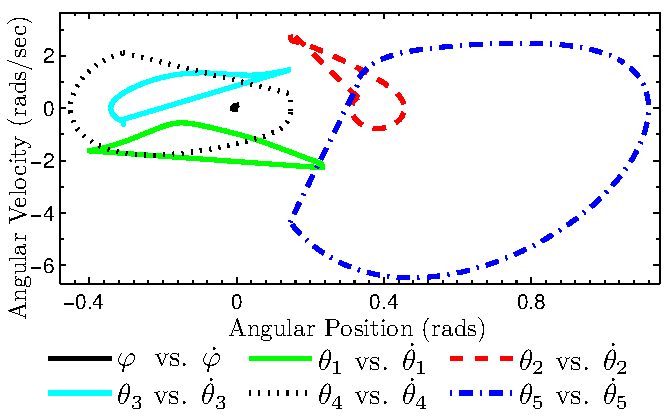
\includegraphics[width=.4\textwidth]{hic_frr_pp_3d_theta}\quad
      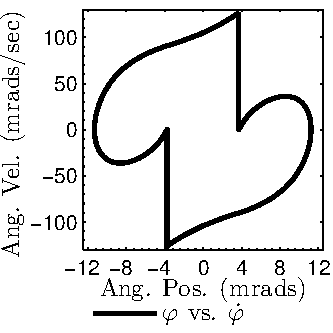
\includegraphics[width=.25\textwidth]{hic_frr_pp_3d_phi}\\[.3em]
      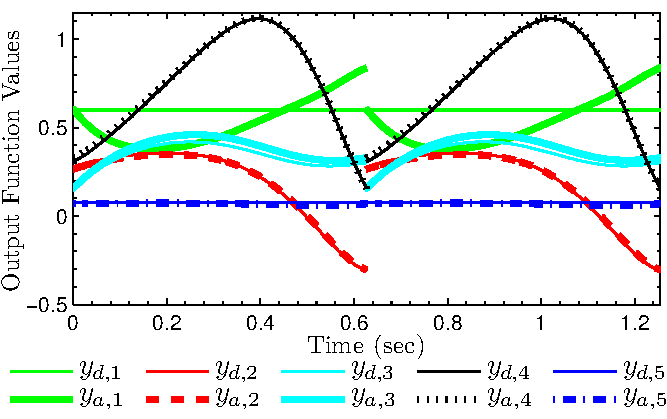
\includegraphics[width=.4\textwidth]{hic_frr_outputs_3d}\quad
      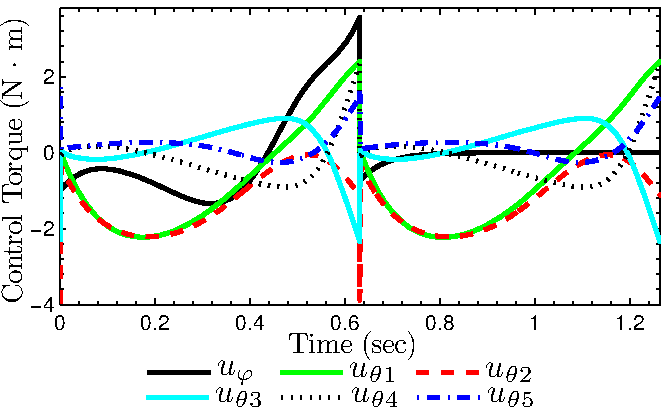
\includegraphics[width=.4\textwidth]{hic_frr_torques_3d}
    \end{figure}
  }
\end{frame}

\begin{frame}
  \frametitle{3D Experiment Results}
  \begin{figure}
    \centering
    \caption{Experimental validation of HIC/FRR scheme}
    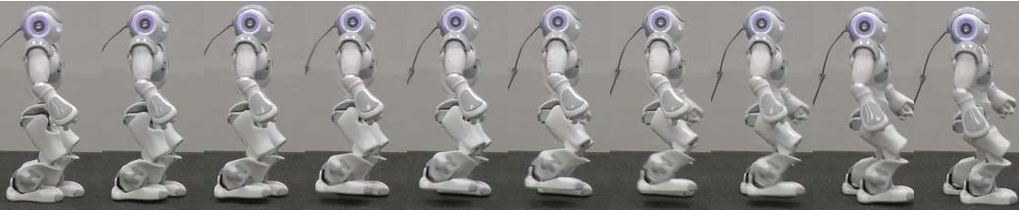
\includegraphics[height=2cm]{nao_tiles}\\[.3em]
    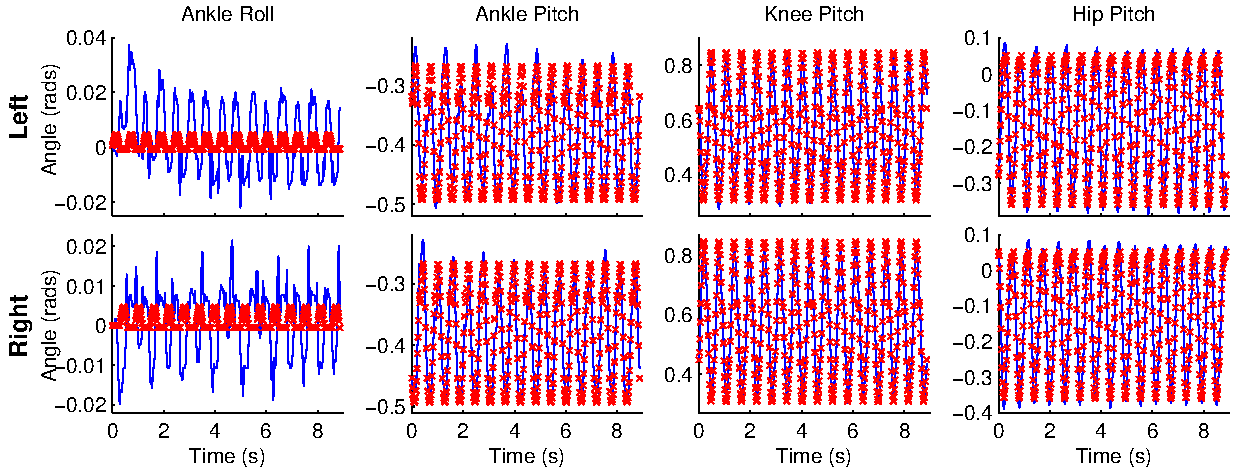
\includegraphics[height=3.25cm]{exp_angles}
  \end{figure}
\end{frame}
